\documentclass[tikz]{standalone}

\begin{document}

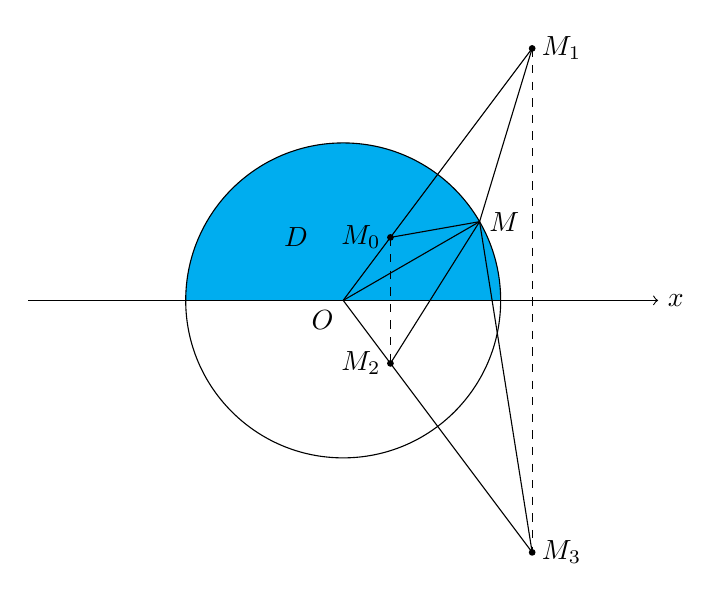
\begin{tikzpicture}[scale=2]
  \fill[cyan] (-1,0) arc[start angle=180, end angle=0, radius=1cm] -- (-1,0);
  \draw (0,0) node[below left] {$O$} circle [radius=1cm];
  \draw[->] (-2, 0) -- (2, 0) node[right] {$x$};
  \draw[fill] (0,0) -- (0.3, 0.4) circle[radius=.5pt] node[left] {$M_0$}
    -- (1.2, 1.6) circle[fill,radius=.5pt] node[right] {$M_1$};
  \draw[fill] (0,0) -- (0.3,-0.4) circle[radius=.5pt] node[left] {$M_2$}
    -- (1.2,-1.6) circle[fill,radius=.5pt] node[right] {$M_3$};
  \draw (0.3, 0.4) -- (30: 1) -- (1.2, 1.6);
  \draw (0.3,-0.4) -- (30: 1) -- (1.2,-1.6);
  \draw[dashed] (0.3, 0.4) -- (0.3,-0.4);
  \draw[dashed] (1.2, 1.6) -- (1.2,-1.6);
  \draw (0,0) -- (30: 1) node[right] {$M$};
  \node at (-0.3, 0.4) {$D$};
\end{tikzpicture}

\end{document}